\documentclass{article}
\usepackage[utf8]{inputenc}
\usepackage{minted}
\usepackage{float}
\usepackage{tikz}
\usetikzlibrary{automata,positioning}

\title{Projet IN406 - Évaluation d’expressions booléennes}
\author{DANKOU Mathis et SOURSOU Adrien}
\date{Mai 2019}

\begin{document}
\maketitle
\section*{Question 1 :}
On définit $G$ la grammaire reconnaissant les expressions booléennes :
\vspace{5px}\\*
\begin{math}
    G = (\Sigma,\;V,\;S,\;P)\\
	\Sigma =\{\;0,\;1,\;NON,\;+,\;.,\;\Rightarrow,\;\Leftrightarrow\;\}\\
    V = \{\;E,\;C,\;OP\;\}\\
    S = E\\ 
    P = \{ \\
    \hspace*{7ex} E\rightarrow C\;|\;(E)\;|\;NON \;E\;|\;E\;OP\;E, \\
    \hspace*{7ex} C\rightarrow \;0\;|\;1, \\
    \hspace*{7ex} OP\rightarrow \;+\;|\;.\;|\;\Rightarrow\;|\;\Leftrightarrow \\
    \}
\end{math}

\section*{Question 2 :}
\begin{minted}{C}
typedef enum { CONSTANTE, OPERATEUR, PARENTHESE } e_type;

typedef enum
{
    FAUX = 0, VRAI = 1,
    NON, ET, OU, IMPLICATION, EQUIVALENCE,
    GAUCHE, DROITE
}   e_valeur;

typedef struct token* liste_token;
struct token
{
    e_type type;
    e_valeur valeur;
    liste_token suivant;
};
\end{minted}

\section*{Question 3 :}
Soient $L$ le langage ainsi que $c$ et $e$ deux expressions régulières : \\
$c$ = $[\;NON\;|\;(^*\;]^*\;[\;0\;|\;1\;]\;)^*$ \\
$e$ = $c\;[\;[\;+\;|\;.\;|\;\Rightarrow\;|\;\Leftrightarrow\;]\;c\;]^*$ \\
$L = \{\; w \in e,\; n\; \geq 0,\; |w|_{(} = |w|_{)} = n\;\}$
\begin{figure}[H]
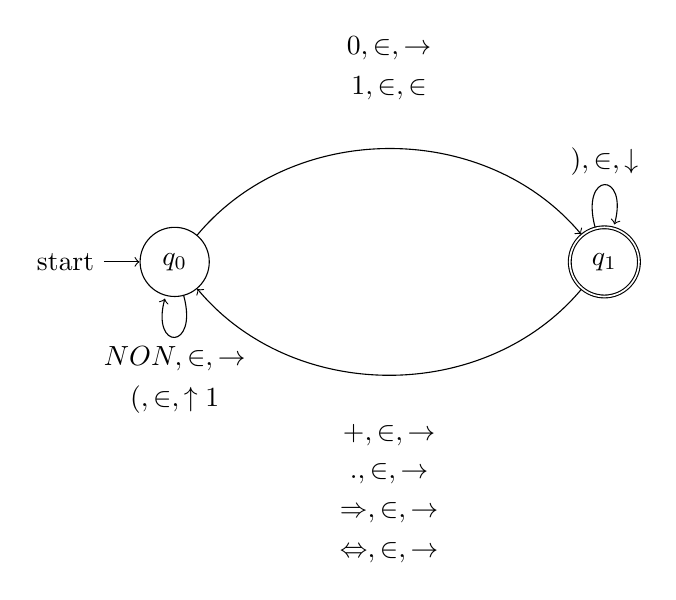
\begin{tikzpicture}
   \node[state,initial] (q_0)  {$q_0$}; 
   \node[state, accepting] (q_1) [right=5cm] {$q_1$}; 
    \path[->] 
    (q_0)   edge [loop below] node[below=0.0] {$NON,\in,\rightarrow$}
                              node[below=0.5] {$(,\in,\uparrow1$} ()
            edge [bend left=50] node[above=1] {$0,\in,\rightarrow$}
                                node[above=0.5] {$1,\in,\in$} (q_1)
    (q_1)   edge [loop above] node {$),\in,\downarrow$} ()
            edge [bend left=50] node[below=0.5] {$+,\in,\rightarrow$}
                                node[below=1] {$.,\in,\rightarrow$}
                                node[below=1.5] {$\Rightarrow,\in,\rightarrow$}
                                node[below=2] {$\Leftrightarrow,\in,\rightarrow$} (q_0);

\end{tikzpicture}
\caption{Automate à pile reconnaissant le langage par état final et pile vide.}
\end{figure}
Définition formelle : \\
\vspace{5px}\\*
\begin{math}
    A = (\Sigma,\;Q,\;\Gamma,\;q_0,\;F,\;T)\\
	\Sigma =\{\;0,\;1,\;NON,\;+,\;.,\;\Rightarrow,\;\Leftrightarrow\;\}\\
	Q = \{\;q_0,\;q_1\;\}\\
    \Gamma = \{\;1\;\}\\
    F = \{\;q_0\;\}\\
    T = \{ \\
    \hspace*{7ex} (q_0,\;\in,\;NON,\;q_0,\;\rightarrow),\;(q_0,\;\in,\;(,\;q_0,\;\uparrow1), \\
    \hspace*{7ex} (q_0,\;\in,\;0,\;q_1,\;\rightarrow),\;(q_0,\;\in,\;1,\;q_1,\;\rightarrow), \\
    \hspace*{7ex} (q_1,\;\in,\;+,\;q_0,\;\rightarrow),\;(q_1,\;\in,\;.,\;q_0,\;\rightarrow), \\
    \hspace*{7ex} (q_1,\;\in,\;\Rightarrow,\;q_0,\;\rightarrow),\;(q_1,\;\in,\;\Leftrightarrow,\;q_0,\;\rightarrow), \\
    \hspace*{7ex} (q_1,\;\in,\;),\;q_1,\;\downarrow), \\
    \}
\end{math}

\section*{Question 4 :}
\begin{minted}{C}
typedef struct arbre* arbre_token;
struct arbre
{
    e_type type;
    e_valeur valeur;
    arbre_token gauche;
    arbre_token droite;
};
\end{minted}

\section*{Question 5 :}
\begin{minted}{C}
int resoudre(e_valeur a, e_valeur b, e_valeur op)
{
    if (op == NON)
        return ! a;
    else if (op == OU)
        return a | b;
    else if (op == ET)
        return a & b;
    else if (op == IMPLICATION)
        return (! a) | b;
    // else (op == EQUIVALENCE)
    return ! a ^ b;
}

int arbre_to_int(arbre_token at)
{
    if (! at)
        return 0;
    else if (at->type == CONSTANTE)
        return at->valeur;
    return resoudre(arbre_to_int(at->gauche), arbre_to_int(at->droite), at->valeur);
}
\end{minted}
\newpage
\section*{Question 7 :}
La priorité des opérateurs est décrite par le tableau de priorité ci-dessous :
\vspace{5px}

\begin{tabular}[h]{|r|l|}
\hline 
    Opérateur & Priorité\\ 
\hline 
    NON & 1\\
\hline 
    . & 2\\
\hline 
    + & 3\\
\hline 
    $\Rightarrow$ & 4\\
\hline 
    $\Leftrightarrow$ & 5\\
\hline
\end{tabular}
\section*{Commentaires}
Le programme par défaut n'affiche que le résultat de l'expression. Cependant, une variable DEBUG peut être modifiée dans le fichier \textit{eval.c} afin de visualiser l'arbre construit.

\vspace{5px}
En plus de la fonction \textit{liste\_token\_to\_arbre\_token}, nous utilisons la fonction \\ \textit{liste\_token\_to\_postfixe}, permettant de transformer notre liste de tokens en liste postfixe.
Au sein de la fonction \textit{liste\_token\_to\_arbre\_token}, les éléments de type constante de la liste sont ajoutés à une pile d'arbre\_token implémentée sous forme de tableau. Les arbres sont combinés ensemble lorsqu'un token de type opérateur est rencontré.

\vspace{5px}
La conversion de la chaîne de caractère en liste de tokens se fait en un seul parcours. \\
La liste de tokens est ensuite parcourue à quatre reprises : une première fois afin de la transformer en liste de tokens postfixe, une seconde afin de calculer la taille maximum de notre pile d'arbres, une troisième pour construire notre arbre de tokens, et une dernière pour libérer la mémoire allouée.

\vspace{5px}
On peut ainsi estimer que la complexité de notre programme est en $O(n)$ linéaire.
\end{document}
